\section{Permutations}
\lecture{2}{5 Sep. 13:10}{}
\begin{prev}
    Instead of choosing the subsets all at once, we could pick one element at a time, then we can try to use product rule.
\end{prev}

\begin{eg}
    Consider
    \[
        \binom{[10]}{3}.
    \]
\end{eg}
\begin{explanation}
    At the choice of the first element, we have \(10\) choices, the second one has \(9\) choisce, while the third one has \(8\) choice, but we didn't consider the order of each picked elements.   
\end{explanation}

\begin{definition}
    Given a set \(X\) and \(k \in \mathbb{N} \cup \left\{ 0 \right\} \), a \(k\)-permutation of \(X\) is 
    \begin{itemize}
        \item an ordered choice of \(k\) distinct elements from \(X\). 
        \item a \(k\)-tuple \((x_1, x_2, \dots , x_k)\) with \(x_i \in X\) and \(x_i \neq x_j\) for each \(i \neq j\). 
        \item an injection \(f: [k] \to X\).       
    \end{itemize}    
    where these \(3\) statements are equivalent. 
\end{definition}
\begin{notation}
    \(X^{\underline{k}} = \left\{ k\text{-permutation of } X \right\} \subseteq X^k \) where \(X^k = X \times X \times \dots \times X\) allows repitition of the elements but \(X^{\underline{k}}\) don't allow repitition. 
\end{notation}

\begin{note}
    If \(\vert X \vert = n\), then 
    \[
        n^{\underline{k}} = \left\vert X^{\underline{k}} \right\vert.
    \]
\end{note}

\begin{definition}
    \vphantom{text}
    \begin{itemize}
        \item a \(n\)-permutation is a \(n\)-permutation of \([n]\). 
        \item a \(X\)-permutation is a \(\left\vert X \right\vert \)-permutation of \(X\).      
    \end{itemize}
\end{definition}

\begin{theorem}[Generalized Product Rule] \label{thm: GeneralizedProductRule}
Suppose we are enumerating \(S\), and can uniquely determine an element \(s \in S\) through a series of \(k\) questions, if \(i\)-th problem always has \(n_i\) possible outcomes, independently to the permutation, then     

\[
    \vert S \vert = n_1 \times n_2 \times \dots \times n_k = \prod_{i=1}^{k} n_i
\]
\end{theorem}
\begin{proof}
    Can make a bijection from \(S\) to 
    \[
        [n_1] \times [n_2] \times \dots \times [n_k].
    \] 
    Map each element in \(S\) to the index of its answer in the series of answer. 
    
    Our moral is when counting we don't care about what the options are but only how many options. 
\end{proof}

\begin{proposition}
\begin{align*}
    n^{\underline{k}} &= n(n-1)\dots (n - (k-1)) \\
    &= \prod_{i=0}^{k-1}(n-i) = \frac{n!}{(n-k)!}.
\end{align*}
\end{proposition}
\begin{proof}
    Use the generalized product rule. 

    Question \(i\): What is the \(i\)-th element in the \(k\)-permutation of \([n]\)? 
    
    We can choose anything except what we're alreafy chosen, so there are \(i-1\) forbidden choices and thus there are \(n-(i-1)\) possible choices.  
\end{proof}

\begin{proposition}
    For all \(0 \le k \le n\), 
    \[
        \binom{n}{k} = \frac{n^{\underline{k}}}{k^{\underline{k}}} = \frac{\left( \frac{n!}{(n-k)!} \right) }{k!} = \frac{n!}{k!(n-k)!}.
    \] 
\end{proposition}
\begin{proof}
    Double-count \([n]^{\underline{k}}\) i.e. \(k\)-permutation of \([n]\). 
    \begin{itemize}
        \item Direct counting \(\left\vert [n]^{\underline{k}} \right\vert = n^{\underline{k}} \). 
        \item First choose the \(k\) elements to appear in the \(k\)-permutation, \(\binom{n}{k}\) options, then choose the order in which they appear, \(k^{\underline{k}}\) options. 
        
        Then, by the generalized product rule, the number of \(k\)-permutation of \([n]\) is \(\binom{n}{k} \cdot k^{\underline{k}}\).   
    \end{itemize}   
    Hence,
    \[
        n^{\underline{k}} = \left\vert [n]^{\underline{k}} \right\vert = \binom{n}{k} \cdot k^{\underline{k}}.
    \] 
\end{proof}

\begin{corollary}
    We can then use this result to reprove Pascal's Property again.
\end{corollary}
\begin{proof}
    
\end{proof}

\begin{exercise}
    \(6\) players at the tennis club want to have three matches involving all the players? How many ways can we arrange the games. 
\end{exercise}
\begin{figure}[H]
    \centering
    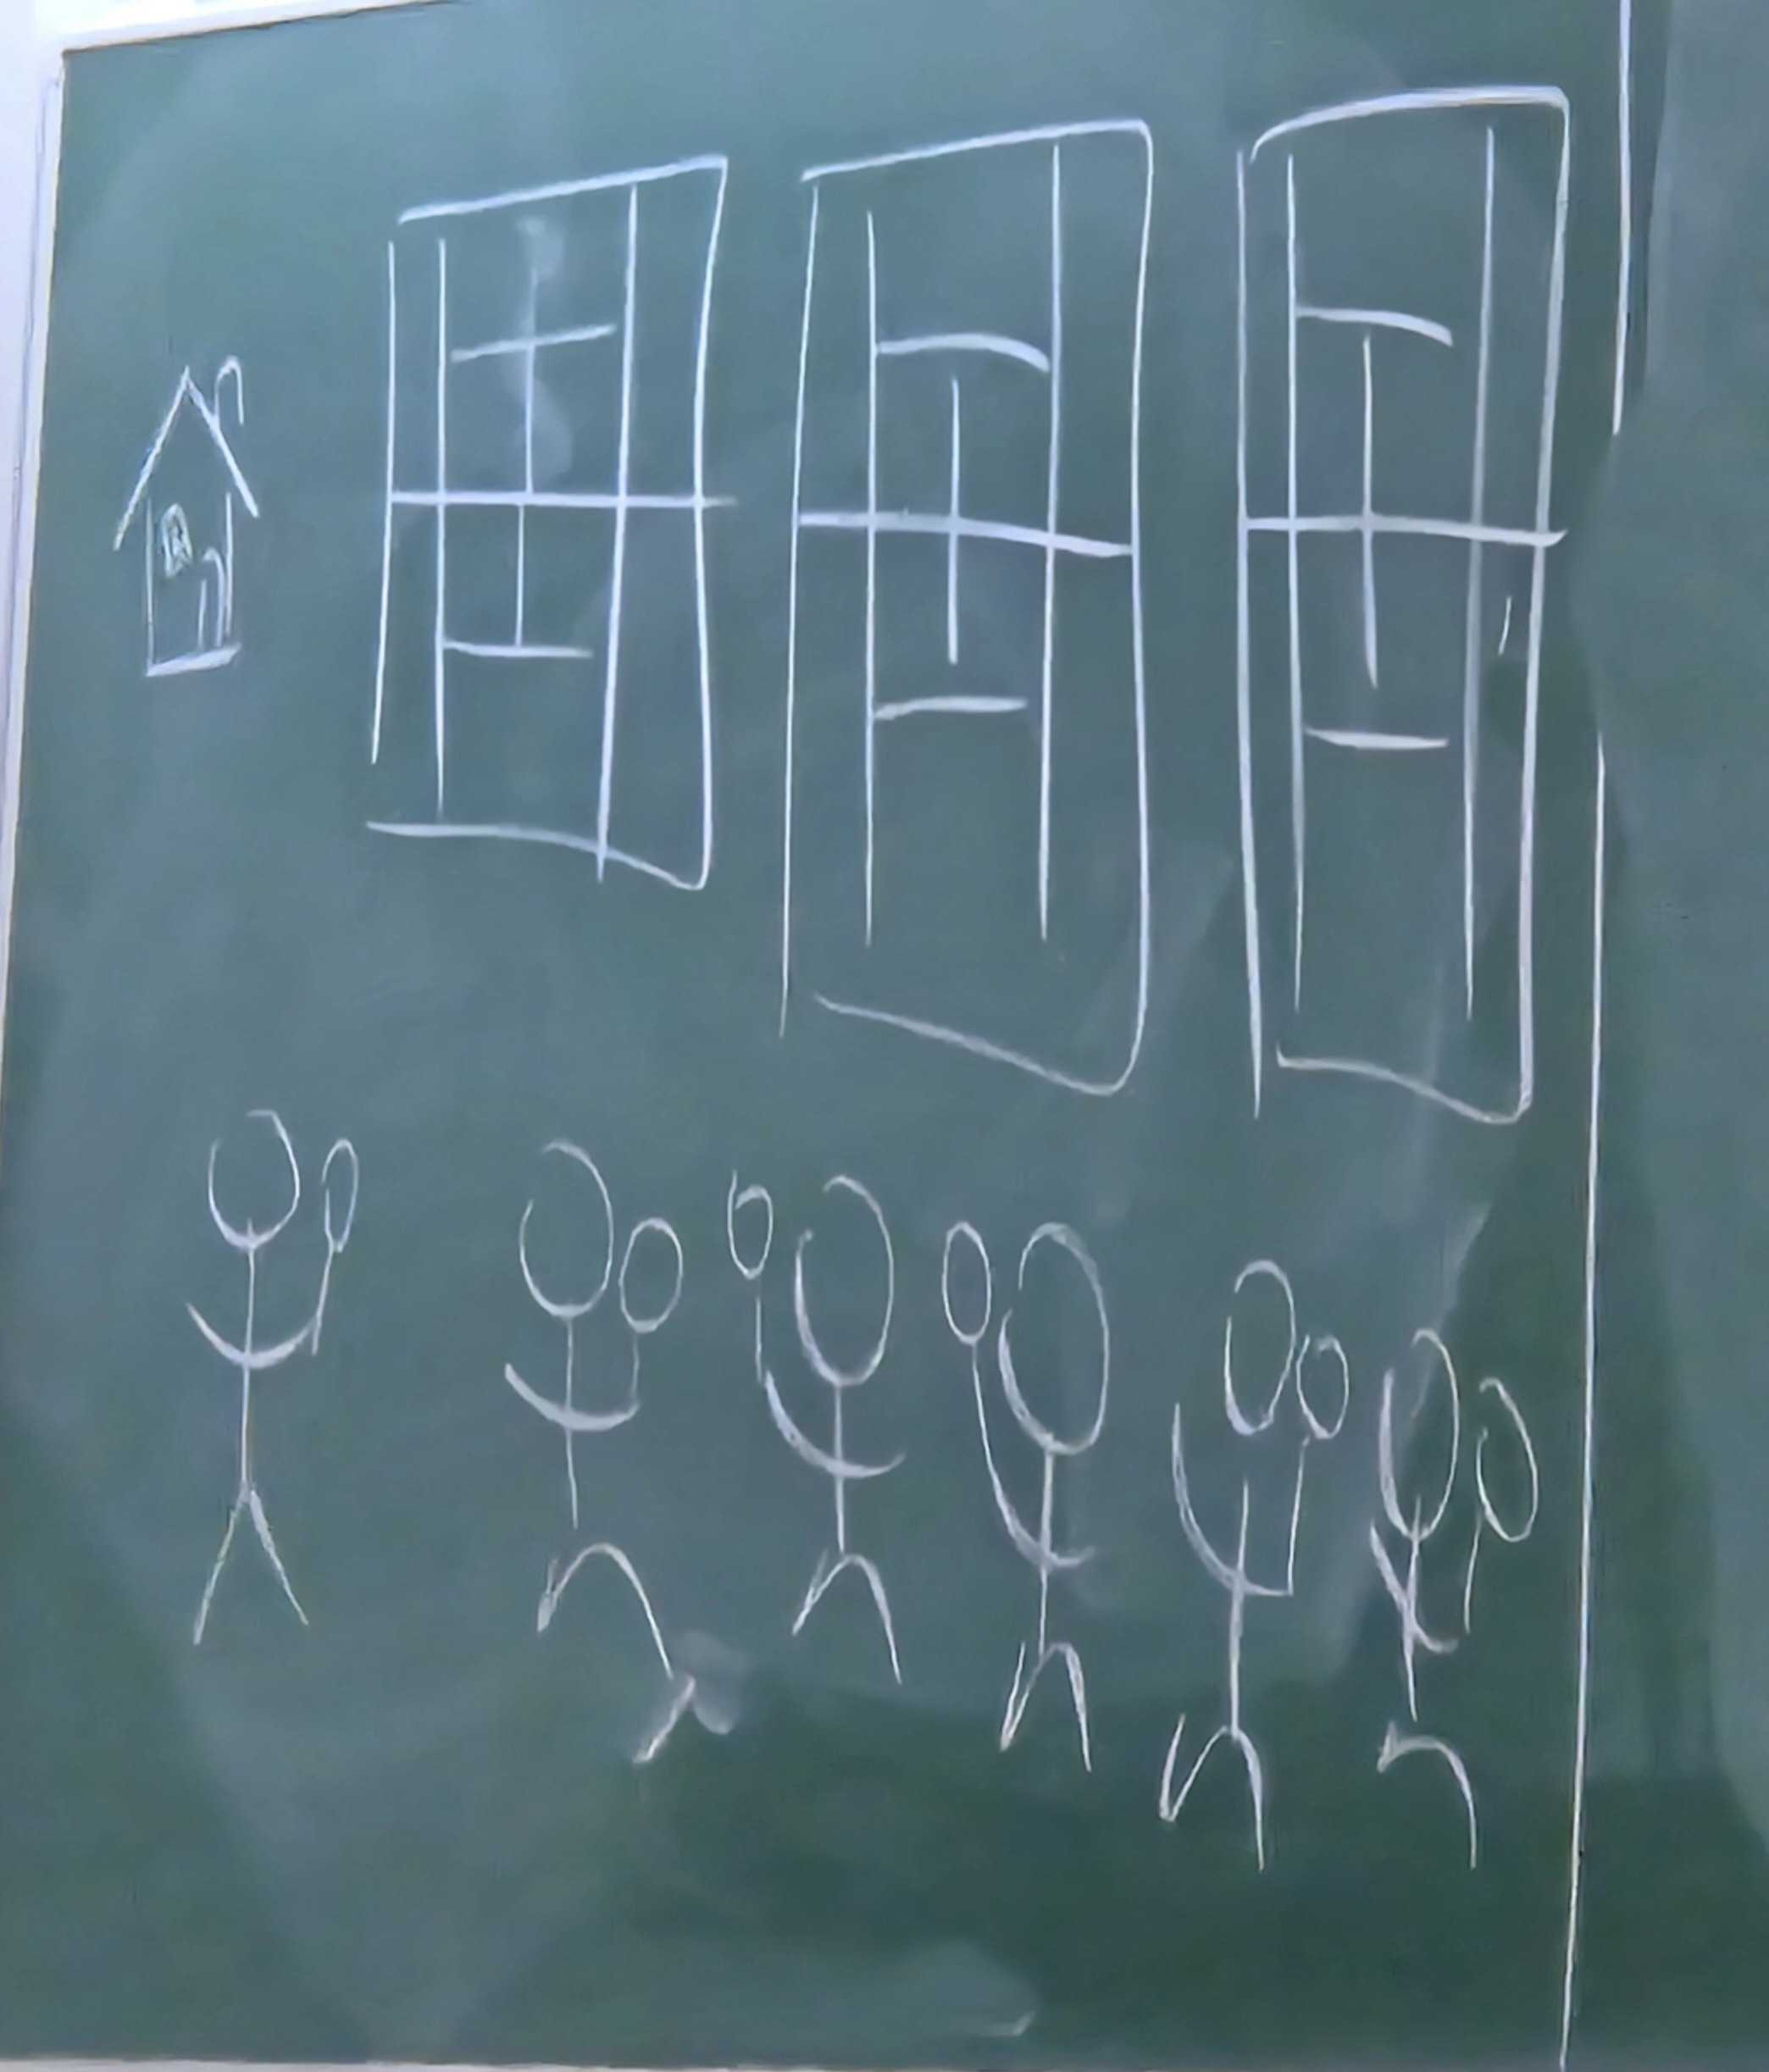
\includegraphics[width=0.4\textwidth]{./Figures/20250905_130141.jpg}
    \caption{Tennis Games}
    \label{fig:tennis game}
\end{figure}
\begin{proof}
    We only care about who plays against whom, not about which court or who versus first, e.t.c. 

    The arrangement of games is a set of three disjoint pairs of players. 
    \[
        \left\{ \left\{ 1,2 \right\} , \left\{ 3,4 \right\} , \left\{ 5,6 \right\}    \right\} \neq \left\{ \left\{ 1,3 \right\}, \left\{ 2,4 \right\}, \left\{ 5,6 \right\}    \right\}. 
    \]

    Double-count the arrangements of games where counts do matter. 
    \begin{itemize}
        \item Choose a pair of players for Court A: \(\binom{6}{2}\)
        \item Choose a pair of players for Court B: \(\binom{4}{2}\)
        \item Choose a pair of players for Court C: \(\binom{2}{2}\) 
    \end{itemize}

    Generalized product rule tells 
    \[
        \text{number of choices} = \binom{6}{2} \binom{4}{2} \binom{2}{2} = 90.
    \]

    Second count: First gets a set of \(3\) pairs, say there are \(x\) possibilities , and assign the three pairs to \(3\) courts, so there are \(3!\) , so \(x \cdot 3! = 90\), and thus \(x = \frac{90}{3!} =15\).  
\end{proof}
